\subsection{常见NLP任务}

\subsubsection{命名实体识别}
NLP中的命名实体识别(Named Entity Recognition)指的是将识别出文本中描述实体的词汇,比如人名、地名、组织机构名、股票基金、医学术语等,更一般地讲,不同的领域会有不同的实体,用于描述该领域内的实体对象。NER的目的就是识别出文本中实体与其他文本的边界和实体的类别。主要以下几个难点:
\begin{itemize}
	\item 实体的数量是无穷的。不同的领域会有不同的实体,且实体并不是定量的,会不断的增加
	\item 实体的构词灵活。同一个实体可能会有多个名字,比如实体的简写;实体也可能是嵌套形成的
	\item 类别模糊。同一个实体在不同的语境下可能会有不同的类别
\end{itemize}

命名实体的识别,从某个角度来看可以视作一个序列标注问题。具体做法是将命名实体附着到{B, M, E, S}标签。其实,词性标注问题也可以以这样的方法来处理。更一般地看,词性标注与命名实体识别是同一个问题,它们都需要对文本进行分词,词性标注中的词性和NER中的实体类别是等价地。

\subsubsection{语法分析}
分析句子中的语法结构并将其表示为容易理解的结构(通常为树形结构)。
\paragraph{短语结构树}根据上下文无关文法将句子/短语分解为树状结构。短语结构语法(上下文无关文法)描述了如何自定向下地生成一个句子,同样句子/短语也可以通过短语结构语法进行分解。这其实和编译原理中的上下文无关文法是很类似的,也是通过很多产生式进行推导,那么是否可以使用编译原理中的词法分析来解决这个问题呢?

\paragraph{依存句法树}关注的是句子中词语之间的语法关联系,并将其约束为树形结构。在句子中,如果一个词语修饰另一个词语,则称修饰词为从属词,被修饰词为支配词,两者之间的语法关系称为依存关系,在可视化时,由支配词指向从属词。依存句法树描述了句子中的各个词之间的依赖关系,一般约定同一个词不能依存于多个词。

\textbf{复合性原理}:一个复杂表达式的意义是由其各组成部分的意义以及结合它们的规则决定的。通过将句子分解为短语、分解短语为单词,下游应用会得到更多更深层次的结构化信息。

\subsubsection{序列标注}
通常也可以看作是token级别的分类问题:对每一个token进行分类。token级别的分类任务通常指的是为为文本中的每一个token预测一个标签结果,如命名实体识、词性标注等。
\begin{itemize}
	\item NER (Named-entity recognition 名词-实体识别) 分辨出文本中的名词和实体 (person人名, organization组织机构名, location地点名...).
	\item POS (Part-of-speech tagging词性标注) 根据语法对token进行词性标注 (noun名词, verb动词, adjective形容词...)
	\item Chunk (Chunking短语组块) 将同一个短语的tokens组块放在一起。
\end{itemize}

\subsubsection{问答系统}
问答式信息检索是一种允许用户以自然语言方式询问,系统从单语或多语文档集中查找并返回确切答案或者蕴含答案文本片断的新型信息检索的方式。问答系统分类如Fig.\ref{fig:qa}所示。
\begin{figure}[h]
	\centering
	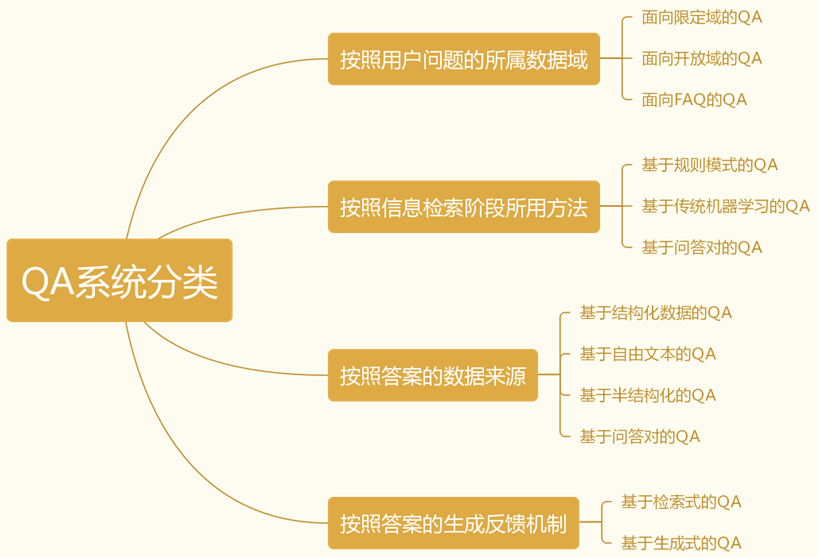
\includegraphics[width=.7\textwidth]{pics/qa.png}
	\caption{问答系统分类,源图\href{https://blog.csdn.net/sinat_33231573/article/details/83473741}{出处}}
	\label{fig:qa}
\end{figure}






\subsection{统计自然语言处理}
\subsubsection{马尔科夫链/隐马尔科夫链}
马尔可夫模型主要用于研究时间序列的分布的,若已有一个是时间序列:$X_0, X_1, X_2, ..., X_n$,马尔可夫模型要解决的就是这些随机变量的取值是如何随着时间而变化的、每个随机变量取值的概率 --- 这些随机变量取值的分布。随机变量的取值可以称为状态。那么问题就成了:
$$
P(X_0=s_0, X_1=s_2, ..., X_n=s_m) = ?
$$
或者说,下一个时刻的随机变量的取值问题:
$$
P(X_n | X_0=s_0, X_1=s_2, ..., X_{n-1}=s_{m-1}) = ?
$$
为了简化这个问题,有了马尔科夫假设。

(1阶)马尔可夫假设:当前状态的取值只取决于前一个时刻的状态。即:
$$
P(X_n | X_0=s_0, X_1=s_2, ..., X_{n-1}=s_{m-1}) = P(X_n | X_{n-1}=s_{m-1})
$$
满足这样性质的一系列随机变量串联在一起就是马尔科夫链了。

那隐马尔科夫链与马尔科夫链又有什么关系呢?
隐马尔科夫模型描述的是两个时序序列的联合分布:$p( \boldsymbol{X}, \boldsymbol{Y} )$,其中$\boldsymbol{X}, \boldsymbol{Y}$均为时序序列,通常称$\boldsymbol{X}$为观测序列,$\boldsymbol{Y}$为状态序列 --- 不可观测序列。其中观测序列/状态序列均可视为随机变量序列(注意,同一时刻的观测变量和状态变量并不是独立的),观测变量序列的取值为可观测值,状态变量序列的取值为状态值 --- 与马尔可夫模型中的状态含义一致。隐马尔科夫模型的假设:
\begin{itemize}
	\item 当前状态变量$\boldsymbol{Y}_t$的取值仅以来与前一个状态变量$\boldsymbol{Y}_{t-1}$的取值有关,连续多个状态变量的取值则构成隐马尔科夫链
	\item 任意时刻的观测变量$\boldsymbol{X}_t$取值仅依赖于该时刻的状态变量的取值$\boldsymbol{Y}_t$
\end{itemize}

一个隐马尔科夫模型可以表示为:$\lambda = (\boldsymbol{\pi}, \boldsymbol{A}, \boldsymbol{B})$,含义如下:
\begin{itemize}
	\item $\boldsymbol{\lambda}$:初始状态概率向量,即初始时刻的状态变量$\boldsymbol{Y}_0$取值为各个状态的概率
	\item $\boldsymbol{A}$:状态转移概率矩阵,即上一时刻的状态变量取某值时,当前时刻状态变量取值的概率分布:$p(\boldsymbol{Y}_t=s_j | \boldsymbol{Y}_{t-1}=s_i)$
	\item $\boldsymbol{B}$:发射概率矩阵,即当前状态变量取某值时观测变量取某观测值的概率分布:$p(\boldsymbol{X}_t=o_j | \boldsymbol{Y}_t=s_j)$
\end{itemize}

其实,可以看出马尔可夫模型是隐马尔科夫模型的一个特例 --- 状态变量序列与观测变量序列相同,状态值即为观测值,每个状态只对应一个观测值即本身。

隐马尔可夫模型的三个应用:
\begin{itemize}
	\item 样本生成问题:给定模型$\lambda = (\boldsymbol{\pi}, \boldsymbol{A}, \boldsymbol{B})$,生成满足模型约束的样本 --- 观测序列即对应的状态序列
	\item 模型的训练:给定训练数据 --- 观测序列即对应的状态序列,估计模型参数$\lambda = (\boldsymbol{\pi}, \boldsymbol{A}, \boldsymbol{B})$
	\item 序列预测:已知模型参数$\lambda = (\boldsymbol{\pi}, \boldsymbol{A}, \boldsymbol{B})$,给定观测序列,求状态序列
\end{itemize}

怎么解决上述的三个问题呢?

对于样本生成问题,其实很简单,指要逐步采样状态,得到一个状态序列,在根据每一步的状态取值采样得到观察值,就可以得到观测序列,样本生成就完成了。

对于模型的训练问题,需要估计的参数为:$(\boldsymbol{\pi}, \boldsymbol{A}, \boldsymbol{B})$,对于$\boldsymbol{\lambda}$则统计所有的状态序列中,计算以每个状态为开头的序列的频率即可,其他两个概率矩阵的训练类比即可。

对于序列预测问题可以通过维特比算法解决。给定一个观测序列,求解最有可能的状态序列。本质上这是一个搜索问题,搜索最有可能的状态序列,使观测序列的似然概率最大。简要地说一下。

维特比算法通过动态规划的方法解决这个问题。假设我们已经有最优的状态路劲,那么其中一条从起点开始的子路径也是最优的子路径。因此可以通过维护两个动态规划的矩阵来记录路径的选择和其概率。假设有两个矩阵$\boldsymbol{\sigma}, \boldsymbol{\psi}$。其中$\boldsymbol{\sigma}_{ti}$表示在时刻$t$时以$s_i$结尾的所有局部路径的最大概率,$\boldsymbol{\psi}_{ti}$表示在时刻$t$时末状态为$s_i$的前驱状态。

\paragraph{应用}使用隐马尔科夫模型可以解中文分词问题。给定训练数据 --- 每个样本为一个句子,对于每个样本,目标是给每个词分配一个标签(如{B, M, E, S}),然后可以根据序列对句子进行分词。为达成这个目的,需要训练隐马尔科夫模型,获得模型的各个参数,根据训练数据是否被标注可以使用不同的方法进行训练。获得训练数据后即可使用模型进行序列预测任务,再根据序列进行分词。


\colorbox{red}{注:本节内容主要参考何晗所著《自然语言处理入门》}。


\subsubsection{概率图模型}
将联合概率分布以图的形式来表示,可以分为有向概率图模型和无向概率图模型。
概率图模型中,将随机变量表示为结点,相关联的随机变量之间会有边连接。

有向图模型中按变量的因果关系进行连接,可以刻画变量之间的因果关系。有向图表示的联合概率可以根据图中的变量依赖关系分解成多个条件概率的积。(听着有点像拓扑图)

无向图模型没有体现出因果关系,强调的是变量之间的相互关系。无向图模型将联合概率分布分解为“无向图中-最大团上-随机变量的函数-的乘积”。



\subsubsection{TF-IDF}
词频-倒排文档频次。通常用于衡量一个词语在文档中的重要程度。单单使用词频评价词语重要程度是不全面的,有些词可能会在文档中出现很多次,但是如果其在很多文档中都出现,却又体现不了其重要性。因此,需要一个对词频进行扩充,希望得到的重要的词应该是这样的:词频高,同时又不是出现在大部分文档中。
$$
TF-IDF(t, d) = \frac{TF(t, d)}{DF(t)} = TF(t, d) \cdot IDF(t)
$$
其中,$TF(t, d)$表示词$t$在文档$d$中出现的次数,$DF(t)$表示包含词$t$的文档数。实际中计算$TF-ID$时会加入一些平滑操作(如加一平滑、对IDF取对数)防止结果下溢等。 IDF表示inverse document-frequency,计算方法:
$$
IDF(t) = \log \frac{1 + n}{1 + DF(t)}
$$
\begin{center}
	或
\end{center}
$$
IDF(t) = \log \frac{n}{1 + DF(t)} + 1
$$
计算得到一个矩阵,每一行表示一个文档的tf-idf向量,每个元素表示对应的词(term)在该文档种的重要程度,一般还会进行$l2$正则化。

\subsubsection{词袋模型}
用于表示文档/句子(其实句子可以看作只有一个句子的文档)的一种方法。
词袋模型一般会先构建一个词表,每个文档经过分词后,可以使用不同的统计量来构建文档/句子的向量,词表之外的词不予考虑。可以选用的不同的统计量有:
\begin{itemize}
	\item 词频
	\item 布尔词频
	\item TF-IDF
	\item 词向量
\end{itemize}

\subsubsection{使用朴素贝叶斯分类器进行文本分类}
首先,给定类别数为$c$,每个文档的特征向量长度为$n$。

朴素贝叶斯分类器是一个生成式的分类器,其计算的是$p(Y | X)$,对于生成模型,重要的是要学习联合分布$p(X, Y)$,朴素贝叶斯通过训练数据学习该联合分布:$p(X, Y) = p(Y)p(X|Y)$。对于给定样本$X^i$,对其进行分类可形式化为:
$$
y = \mathop{argmax}_{c_k} p(Y=c_k | X=X^i) = \mathop{argmax}_{c_k} \frac{p(X=X^i | Y=c_k) p(Y=c_k)}{p(X=X^i)}
$$
朴素贝叶斯中假设样本的特征之间是相互独立的,即$p(X)=p(X_1=x_1, ..., X_n=x_n) = p(X_1=x_1) ... p(X_n=x_n)$。那么为了得到样本$X^i$的类别,只需要计算出$p(X=X^i | Y=c_k),  p(Y=c_k), p(X=X^i)$即可。而对于某一个样本的分类,$p(X^i)$对分类是没有帮助的,在$Y$取不同类别时是不会变化的,故可以不计算$p(X^i)$。那么剩下的需要计算的只有出$p(X=X^i | Y=c_k),  p(Y=c_k)$了。

$p(Y=c_k)$是很好计算的,只需要统计训练数据中类别为$c_k$的样本所占的比例即可。由于特征之间独立的假设,所以$p(X^i | Y=c_k) = \prod_{j=1}^{n} p(X_{j}^{i}=x_j | Y=c_k)$。这个概率也只需要从训练数据中统计即可,统计每个类别下,特征向量的第$j$维取$x_j$的比例即可。

关于样本的特征向量:通常可以采用词袋模型的方法来表示一个文本/句子。


\subsubsection{预训练}
预训练在很多领域上都有应用,如CV、NLP。当用深度学习来解决一个任务时,使用的深度模型通常会包含很多参数,我们需要使用大量的数据来更新我们的参数使之能够在特定的任务上取得不错的效果。一般,我们会对模型的参数初始化,然后使用大量带标签的数据来更新模型参数。

但实际情况是,带标签的数据总是很少的。

\begin{figure}[h]
	\centering
	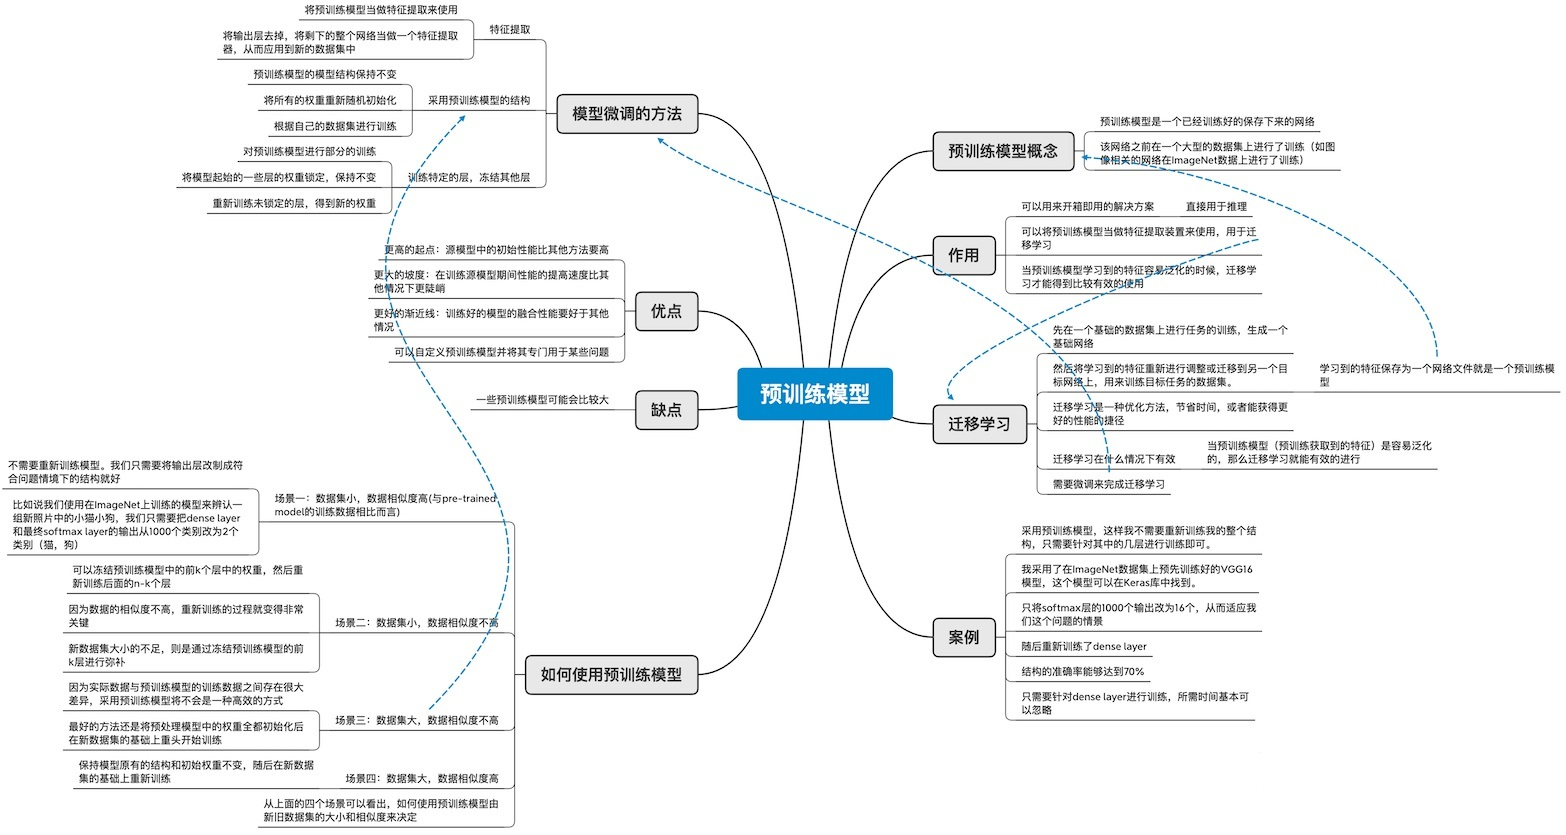
\includegraphics[width=\textwidth]{pics/pre-train.jpg}
	\caption{预训练模型(\href{https://www.zhihu.com/question/327642286/answer/1215812016}{出处})}
	\label{fig:pre-train}
\end{figure}
预训练通常在大量无监督的数据上学习(可以是无监督的学习任务、简单的有监督学习任务),用无监督的数据帮助模型的参数收敛,后续再在监督数据上进行调整。


\subsection{Deep Model for NLP}

\subsubsection{Transformer}
在NLP中有很多输入为序列输出为序列的\textbf{seq2seq}任务,例如机器翻译、文本摘要、序列标注、文本生成等等。早期的seq2seq任务RNN-based\cite{sutskever2014sequence, cho2014learning}模型为主,但RNN-based的模型容易出现以下问问题:
\begin{itemize}
	\item RNN处理seq2seq任务时通常将输入序列转换成一个context向量,再基于context来得到输出的序列。单个向量难以包含输入序列的所有信息
	\item RNN在递归的解码过程使得其难以处理长文本序列
	\item RNN的反向传播容易出现梯度弥散/爆炸问题
	\item 序列的处理是串行的,难以并行化,计算效率低
\end{itemize}
\textbf{Attention}\cite{bahdanau2016neural, luong2015effective}技术 --- 帮助RNN-based模型解决了一部分困难。具体是怎么做的呢?在RNN-based模型的基础上主要有以下几个变化:
\begin{itemize}
	\item 编码器传给解码器的不再只是一个context向量,会利用编码过程中的所有隐向量
	\item 解码时,会根据所处的时间步,为每一个隐向量计算一个分数,归一化后再分别与隐向量相乘得到当前时间步的context向量
\end{itemize}

有了Attention,RNN-based模型的一部分缺点得到了解决(处理长文本序列的问题),但还是有一些问题:不能并行化处理输入序列,且能不能直接在Attention上构建seq2seq模型呢?

\textbf{Transformer}\cite{vaswani2017attention}来了!!!
Transformer采用的也是编解码的结构:先对输入序列进行编码,再根据编码的输出进行解码。与RNN-based模型不同的是,其不是递归的处理输入,Transformer可以并行地处理整个文本序列。 

Transformer的模型结构如Fig.\ref{fig:transformer}所示。具体的计算过程可以参考论文\cite{bivaswani2017attentionbid}的论文笔记。
\begin{figure}[h] 
	\centering
	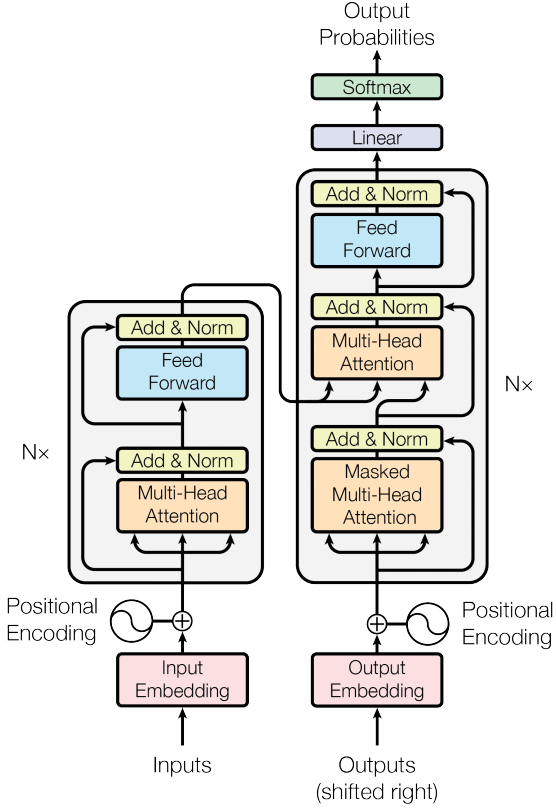
\includegraphics[width=.4\textwidth]{pics/Transformer.png}
	\caption{Architecture of Transformer}
	\label{fig:transformer}
\end{figure}

\begin{itemize}
	\item 由于Transformer没有循环结构,但是加入了Positional Encoding
	\item 编码部分最终的输出。会作为Decoder Block中Attention的$K, V$,解码器的输入作为$Q$
	\item Decoder Block中的Masked Multi-head Attention,处理当前输入时只允许看到当前位置之前的输入
	\item 在编码器中,也有mask。因为通常对输入进行padding
\end{itemize}

\subsubsection{一些关于Transformer的问题}
\paragraph{1.}{\textbf{为什么输入$X$要经过变换得到$Q, K, V$? 为什么不直接使用$X$?}}

如果直接使用$X$,则$X$直接承担了三种角色:查询、键和值。难以学习到满足要求的$X$。经过变换后得到的$Q, K, V$,$Q$负责表示查询的问题,$V$表示输入的信息,$K$表示与输入相关的“关键词”,$Q, K$相乘用于衡量查询的问题与各条信息之间的相似性。

\subsubsection{BERT}
\paragraph{Motivation}
BERT(Bidirectional Encoder Representations from Transformers)\cite{devlin2019bert}缘自Transformer模型。通常的语言模型都是单向的,例如从左到右,这使得在处理每个token时只能利用其之前的token。单向的模型处理token-level的任务时,难以应用到上下文的信息。

\paragraph{HOW?}
BERT在大量无标签的文本数据集进行预训练,得到模型的参数后,再添加具体任务相关的神经网络层,微调后即可得到适用于具体任务的模型,即:pre-training + fine-tuning。

\par{\textbf{Pre-training}}BERT使用两个预训练任务。

\par{\textbf{Fine-tuning}}

\paragraph{title}

\subsection{词嵌入模型}
\subsubsection{Word2Vec}

\subsubsection{ELOM}